\section{Proof of Lemma \ref{lem:key}: computation of a representation of the Kleene closure}

Recall that one important component in the decidability of $\GPtwo$ is the computation of a representation of the Kleene closure of a semilinear set.
Recall from Section \ref{sec:prelims} that $\projp{n}{\bfv}$ denotes the projection operator that maps a vector $\bfv$ to its first $n$ entries.
The formal statement was:

\medskip

For every integer linear system $\cQ(\bfx): \bfA \bfx = \bfc$ with $\bfc \neq \bfzero$,
where $\bfA \in \bbZ^{m \times n}$ and $\bfc \in \bbZ^{m}$,
there exists $\bfAtilde \in \bbZ^{(n+t) \times (n+k)}$ with $\norm{\bfAtilde} = 1$
such that
\begin{equation*}
    \kstar{\sol{\cQ(\bfx)}}\ =\ \sol{\cQtilde(\bfx)},
\end{equation*}
where $\cQtilde(\bfx)$ is the following Boolean combination of integer linear systems
\begin{equation*}    
    \exists \bfy_1, \bfy_2\ 
    (\bfx\ =\ \projp{n}{\bfy_1} + \bfy_2)\ \land\ 
    (\bfAtilde\bfy_1\ =\ \bfzero)\ \land\ 
    (\bfA\bfy_2\ =\ \bfzero)\ \land\ 
    ((\bfy_1=\bfzero) \to (\bfy_2=\bfzero)),
\end{equation*}
$k = n\cdot(2D+1)^{m} + 1$,
$t \le 2nk$, and
$D = n \cdot \norm{\bfA} \cdot \left((n+1)\cdot \norm{\bfA} + \norm{\bfc} + 1\right)^{m}$.
Moreover, $\bfAtilde$ can be computed in time $2^\bigO{\log n + \log K + m^2}$,
where $K := \max\left(\norm{\bfA}, \norm{\bfc}\right)$.

\medskip

We prove the lemma by considering \emph{minimal solutions} of the integer linear system.
Recall that $\vle$ means pointwise inequality between vectors.
\begin{definition}[Minimal elements]
    For a set $\cS \subseteq \bbN^n$ and $\bfv \in \cS$,
    we say that $\bfv$ is \emph{minimal} in $\cS$
    if, for every $\bfu \in \cS$ with $\bfu \neq \bfv$,
     $\bfu \not\vle \bfv$.
\end{definition}

Note that the following properties about minimal elements are trivial.
\begin{lemma}\label{lem:min_property}
    Let $\cS$ be a nonempty subset of $\bbN^n$.
    \begin{enumerate}
        \item There exists $\bfv \in \cS$ such that $\bfv$ is minimal in $\cS$.
        \item For every $\bfv \in \cS$, there exists a minimal element $\bfu \in \cS$,
            such that $\bfv - \bfu \in \bbN^n$.
    \end{enumerate}
\end{lemma}

For an integer linear system $\cQ(\bfx)$,
let $\solmin{\cQ(\bfx)}$ denotes the set of minimal solutions,
i.e., $\solmin{\cQ(\bfx)} := \setc{\bfv \in \sol{\cQ(\bfx)}}{\bfv\ \text{is minimal in}\ \sol{\cQ(\bfx)}}$.
Note that the maximal entry of minimal solutions is bounded.

\begin{lemma}[\cite{Pottier}, also see Proposition 4. in~\cite{semilinear}]\label{lem:minimal}
    For every integer linear system $\cQ(\bfx): \bfA \bfx = \bfc$,
    where $\bfA \in \bbZ^{m \times n}$ and $\bfc \in \bbZ^{m}$,
    for every $\bfv \in \solmin{\cQ(\bfx)}$,
     $\norm{\bfv} \le \left((n+1)\cdot\norm{\bfA} + \norm{\bfc} + 1\right)^{m}$.
\end{lemma}

We begin by turning to the automata-theoretic approach for the solutions of integer linear systems.

\begin{definition}[Acyclic, unambiguous, and simple finite automata] \label{def:simpleplus}
As usual, a finite automaton can be viewed as a 
directed graph where the vertices are the states
and the edges are the transitions.

Such an automaton is \emph{acyclic} if the graph does not contain a cycle. 
It is \emph{unambiguous} if every word has 
at most one accepting run.
    We say that a finite automaton is \emph{simple}
    if it is unambiguous, acyclic, and has exactly one accepting state.
\end{definition}

\begin{definition}[Parikh Vector]
    For a word $w = a_{t_1}\cdots a_{t_\ell} \in \Sigma^*$,
    the \emph{Parikh vector} of $w$
    is a vector in $\bbN^{n}$, defined as
    $\parikh{w} := \sum_{i \in \intsinterval{\ell}} \unit{t_i}$.
    Intuitively, the $i^{th}$ entry in $\parikh{w}$ is the number of occurrences of $a_i$ in $w$.

For a finite automaton $\cM$, the \emph{Parikh image} of $\cM$ is defined as
\begin{equation*}
\parikh{\cM}
\ :=\ 
\setc{\parikh{w}}{\text{$\cM$ accepts $w$}}.
\end{equation*}
\end{definition}

We can encode a finite subset of solutions of a linear system $\cQ(\bfx):\bfA \bfx = \bfc$ as the Parikh image of a finite automaton $\cM$.
More precisely, $\parikh{\cM}$ contains all the minimal solutions of $\cQ(\bfx)$.
The main idea behind the construction of $\cM$ is as follows.
Suppose $\cQ(\bfx)$ has a solution
and $\bfA\in \bbZ^{m\times n}$.
By Lemma~\ref{lem:minimal},
the components of every minimal solution are bounded above by  
$L:=\left((n+1)\cdot\norm{\bfA} + \norm{\bfc} + 1\right)^{m}$.
We can construct a finite automaton $\cM$ where the set of states is $\setc{\bfA\bfv}{\bfv \in [0,L]^n}$
and the transitions are
$\langle \bfA\bfv,a_i, \bfA(\bfv+\bfe_i) \rangle$ for every $1\le i \le n$.
The initial state is $\bfzero$ and the accepting state is $\bfc$.
Obviously, $\parikh{\cM}$ contains all the minimal solutions. In fact, it contains all solutions that are bounded by $L$. 
Note also that
$\cM$ can be constructed in exponential time.
With a little more work, we can make $\cM$ simple, a property that will be useful when analyzing the Kleene star of $\sol{\cQ}$.

\begin{lemma}\label{lem:ilp_to_nfa}
For every integer linear system $\cQ(\bfx): \bfA \bfx = \bfc$,
where $\bfA \in \bbZ^{m \times n}$ and $\bfc \in \bbZ^{m}$,
there exists a simple finite automaton $\cM$
with $k$ states and $t$ transitions,
where $k = n\cdot L\cdot(2D+1)^{m} + 1$, 
$t \le 2nk$,
$L = \left((n+1)\cdot\norm{\bfA} + \norm{\bfc} + 1\right)^{m}$
and $D = n \cdot \norm{\bfA} \cdot L$,
    such that
    \begin{equation*}
        \solmin{\cQ(\bfx)}
        \ \subseteq\ 
        \parikh{\cM}
        \ \subseteq\ 
        \sol{\cQ(\bfx)}.
    \end{equation*}
    Moreover, $\cM$ can be constructed in time exponential in $n,m,\norm{\bfA},\norm{\bfc}$.
\end{lemma}

\begin{proof}
If $\bfc = \bfzero$, then the system $\cQ(\bfx)$ admits the
solution $\bfzero$.
The finite automaton that accepts only the empty word is the desired $\cM$.
So we concentrate on the case when $\bfc\neq \bfzero$.

The automaton $\cM$ is very similar to the one described in the intuition preceding the lemma.
We fix a finite alphabet of $n$ symbols $\Sigma := \set{a_1, \ldots, a_{n}}$.
To ensure acyclicity, we modify the automaton $\cM$ to accept only words from $a_1^*a_2^*\cdots a_n^*$. The automaton will also implement a counter that counts the number of occurrences of each $a_i$ up to $L$. Such a counter can be implemented using the states of $\cM$.
We now give the details.

Let $\cD$ be the set $\intinterval{-D}{D}^{m}$.
\begin{itemize}
\item 
The set of states is 
$\{q_{acc}\}\cup(\intsinterval{n}\times\intsinterval{L} \times \cD)$.
\item
The initial state is $(0,0,\bfzero)$.
\item 
For each $0\leq i<j \leq n$, $0\leq t\leq L-1$,
and $\bfv \in \cD$,
we have the transitions:
\begin{itemize}
\item 
if $\bfv + \bfA\unit{i} \in \cD$,
then $(\tuple{i,t, \bfv}, a_i, \tuple{i,t+1, \bfv + \bfA\unit{i}}) \in \Delta$, 
\item 
if $\bfv + \bfA\unit{i}  = \bfc$,
then $(\tuple{i, t,\bfv}, a_i, q_{acc}) \in \Delta$.

\item 
if $\bfv + \bfA\unit{j} \in \cD$,
then $(\tuple{i,t, \bfv}, a_j, \tuple{j,1, \bfv + \bfA\unit{j}}) \in \Delta$, 
\item 
if $\bfv + \bfA\unit{j}  = \bfc$,
then $(\tuple{i, t,\bfv}, a_j, q_{acc}) \in \Delta$.
\end{itemize}
\end{itemize}
Obviously, $\cM$ has only one accepting state.
The automaton $\cM$ is acyclic since it can only go from the state
$\tuple{i,t, \bfv}$ to $\tuple{j,t',\bfu}$
when $i< j$ or when $i=j$ and $t<t'$.
It is also unambiguous since
for every state $\tuple{i,t,\bfv}$ and $a\in \Sigma$, there is at most one state $\tuple{i',t',\bfu}$
such that $\tuple{i,t,\bfv},a,\tuple{i',t',\bfu}$ is a transition.
Finally, it is routine to verify that
$\parikh{\cM}\subseteq \sol{\cQ}$.
That $\solmin{\cQ}\subseteq \parikh{\cM}$
follows from Lemma~\ref{lem:minimal}.
\end{proof}

Next, we consider the Kleene star of sets.
Recall the definition:

\medskip

For every $\cS \subseteq \bbN^n$,
the \emph{Kleene star} of $\cS$ is defined as
\begin{equation*}
    \kstar{\cS} := \setc{\sum_{s \in \cS'} s}{\text{$\cS'$ is a finite multisubset of $\cS$}}.
\end{equation*}

\medskip

In the following we fix a finite alphabet of $n$ symbols $\Sigma:=\{a_1,\ldots,a_n\}$
and assume that every finite automaton is over this alphabet.
We need more terminology concerning finite automata.
Note that for every acyclic finite automaton $\cM$ (Definition \ref{def:simpleplus})
a run $r$ of $\cM$ uses each transition at most once.
Therefore, we can represent $r$ by a Boolean vector with dimension $\abs{\Delta}$.
Recall that for a unambiguous finite automaton $\cM$ and an accepted word $w$, there exists exactly one accepting run of $\cM$ on $w$.
Let $\bbB:=\{0,1\}$.

\begin{definition}
    For every simple finite automaton $\cM$ with $t$ transitions,
    for every accepted word $w$ of $\cM$,
    letting $r$ be the unique accepting run of $\cM$ on $w$,
    the \emph{path vector} of $w$, denoted by $\mpath{w}$,
    is the vector in $\bbB^t$ defined as follows:
    for $1 \le i \le t$, the $i^{th}$ entry of $\mpath{w}$ is 1
    if and only if $r$ contains the $i^{th}$ transition.
\end{definition}

\begin{lemma}\label{lem:path}
For every simple finite automaton $\cM$ with $t$ transitions,
there exists a matrix $\bfB_\cM \in \bbZ^{n \times t}$,
which can be computed in time $\bigO{nt}$,
such that
\begin{itemize}
\item $\norm{\bfB_\cM} = 1$, and
\item for every word $w$ accepted by $\cM$, $\parikh{w} = \bfB_\cM\cdot\mpath{w}$.
\end{itemize}
\end{lemma}

\begin{proof}
    We construct the matrix $\bfB$ as follows.
    For $1 \le i \le n$ and $1 \le j \le t$,
    if the $t^{th}$ transition is of the form $(q, a_i, p)$,
    then $(B_\cM)_{i, j} = 1$.
    Otherwise, $(B_\cM)_{i, j} = 0$.
    It is trivial to verify that
    $\parikh{w} = \bfB\cdot\mpath{w}$.
\end{proof}

We now prove a  lemma regarding the Kleene closure of the Parikh image.
The proof employs a similar idea as in the argument for Theorem~1 in \cite{tree}.

\begin{lemma}\label{lem:kstar_nfa}
    For every simple finite automaton $\cM$ with $k$ states $q_1, \ldots,q_k$ and $t$ transitions,
    there exists a matrix $\bfA_\cM \in \bbZ^{k \times t}$,
    which can be computed in time $\bigO{kt}$,
    such that
    \begin{itemize}
        \item $\norm{\bfA_\cM} = 1$, and
        \item $\kstar{\parikh{\cM}} =
            \sol{\cQ_\cM(\bfx)}$,
            where
            $\cQ_\cM(\bfx) := \exists \bfy\ (\bfx = \projp{n}{\bfy}) \land (\tilde{\bfA}_\cM \bfy = \bfzero)$ and
            $\bfAtilde_\cM = 
            \left[
                \begin{array}{r|r}
                    -\bfI & \bfB_\cM \\
                    \hline
                    \bfzero& \bfA_\cM
                \end{array}
            \right]$.
    \end{itemize}
\end{lemma}

\begin{proof}
    We construct the matrix $\bfA_\cM$ as follows.
    For $1 \le i \le k$ and $1 \le j \le t$,
    if $q_i$ is the initial state or the accepting state, then
    $\left(A_\cM\right)_{i, j} = 0$.
    Otherwise,
    \begin{equation*}
        \left(A_\cM\right)_{i, j}\ :=\ 
        \begin{cases}
            1,  &\text{if the $j^{th}$ transition is of the form $(p, a, q_i)$} \\
            -1, &\text{if the $j^{th}$ transition is of the form $(q_i, a, p)$} \\
            0,  &\text{otherwise}.
        \end{cases}
    \end{equation*}
    Note that since $\cM$ is acyclic, there is no transition of the form $(q_i, a, q_i)$.

    We first claim that for every accepted word $w$, 
    we have
    \begin{equation*}
        \bfA_\cM \cdot \mpath{w} = \bfzero.    
    \end{equation*}
    We will show that $\left(\bfA_\cM \cdot \mpath{w}\right)_i = 0$,    for $1 \le i \le k$.
    If $q_i$ is the initial state or the accepting state,
    by definition, $\left(A_\cM\right)_{i, j} = 0$ for every $1 \le j \le k$,
    hence, $\left(\bfA_\cM \cdot \mpath{w}\right)_i = 0$.

    If $q_i$ does not appear in the accepting run of $w$,
    then $\mpath{w}_j=0$ if
    the $j^{th}$ transition is going into or coming out of state $q_i$.
    Hence, $\left(\bfA_\cM \cdot \mpath{w}\right)_i = 0$.

    Now, suppose that $q_i$ appears in $\mpath{w}$
    and it is 
    neither the initial state nor the accepting state.
    Let $r$ be the accepting run of $\cM$ on $w$.
    Since $\cM$ is acyclic, $q_i$ appears only once, which implies that $r$ is of the form
    \begin{equation*}
        \cdots p\transs{a} q_i \transs{a'}p'\cdots
    \end{equation*}
    Suppose that
    $\tuple{p, a, q_i}$ is the $j_1^{th}$ transition and 
    $\tuple{q_i, a', p'}$ is the $j_2^{th}$ transition.
    Then we have:
    \begin{equation*}
        \left(\bfA_\cM \cdot \mpath{w}\right)_i
        =
        \left(\bfA_\cM\right)_{i, j_1} +
        \left(\bfA_\cM\right)_{i, j_2}
        = 1 + (-1)
        = 0.
    \end{equation*}

    We will now show that
    $\kstar{\parikh{\cM}} = \sol{\cQ_\cM(\bfx)}$.

    \textbf{\uline{$\kstar{\parikh{\cM}} \subseteq \sol{\cQ_\cM(\bfx)}$}.}
    Suppose that $\bfv \in \kstar{\parikh{\cM}}$.
    By the definition of Kleene star and Parikh image,
    there exist accepted words $w_1, \ldots, w_\ell$
    and $\bfv = \sum_{i \in \intsinterval{\ell}} \parikh{w_i}$.
    Let $\bfu := \sum_{i \in \intsinterval{\ell}} \mpath{w_i}$.
    By the claim above and Lemma~\ref{lem:path}, we have
    \begin{equation*}
        \begin{aligned}
            \bfA_\cM \bfu\ =\ &\sum_{i \in \intsinterval{\ell}} \bfA \cdot \mpath{w_i}\ =\ \bfzero \\
            \bfB_\cM \bfu\ =\ &\sum_{i \in \intsinterval{\ell}} \bfB \cdot \mpath{w_i}
            \ =\ \sum_{i \in \intsinterval{\ell}} \parikh{w_i}\ =\ \bfv,
        \end{aligned}
    \end{equation*}
    which implies that concatenation of $\bfv$ and $\bfu$ is a solution of the integer linear system $\cQ_\cM(\bfx)$.
    Hence, $\bfv \in \sol{\cQ_\cM(\bfx)}$.

    \textbf{\uline{$\sol{\cQ_\cM(\bfx)}\subseteq\kstar{\parikh{\cM}}$}.}
    Suppose that $\bfv \in \sol{\cQ_\cM(\bfx)}$.
    Let $\bfu$ be the vector satisfying $\bfv = \bfB_\cM\bfu$ and $\bfA_\cM\bfu = \bfzero$.
    We interpret the $j^{th}$ entry of $\bfu$, denoted by $u_j$
    as a flow of the $j^{th}$ edge (transition) in the transition diagram of $\cM$.
    Then, since $\bfA_\cM\bfu = \bfzero$ by the claim above,
    for every node (state) $q$,
    if $q$ is neither the initial state nor the accepting state,
    then 
    \begin{equation*}
        \sum_{\substack{
                j \in \intsinterval{t}\\
                \text{the $j^{th}$ transition is of the form $(p, a, q)$}
        }} u_j
        -
        \sum_{\substack{
                j \in \intsinterval{t}\\
                \text{the $j^{th}$ transition is of the form $(q, a, p)$}
        }} u_j
        = 0.
    \end{equation*}
    That is, the incoming flow to the node (state) $q$ equals its outgoing flow.
    By the flow decomposition theorem~\cite{flow},
    there exist paths (words) $w_1, \ldots, w_\ell$ from the initial state to the accepting state
    such that $\bfu = \sum_{i \in \intsinterval{\ell}} \mpath{w_i}$.
    Since each $w_i$ is a path from the initial state to the accepting state, each
    $w_i$ is a word accepted by $\cM$.
    By Lemma~\ref{lem:path}, for each $i \leq \ell$, $\parikh{w_i} = \bfB_\cM\cdot\mpath{w_i}$.
    Thus, we have
    \begin{equation*}
        \bfv
        \ =\ \bfB_\cM\bfu
        \ =\ \sum_{i \in \intsinterval{\ell}} \bfB_\cM\cdot\mpath{w_i}
        \ =\ \sum_{i \in \intsinterval{\ell}} \parikh{w_i}
        \ \in\ \kstar{\parikh{\cM}}.
    \end{equation*}
\end{proof}

Combining Lemma~\ref{lem:ilp_to_nfa} and Lemma~\ref{lem:kstar_nfa} we obtain
a lemma regarding the Kleene star of the set of minimal solutions of an integer linear system.
\begin{lemma}\label{lemma:kleene_minimal}
    For every integer linear system $\cQ(\bfx): \bfA \bfx = \bfc$,
    where $\bfA \in \bbZ^{m \times n}$, $\bfc \in \bbZ^{m}$,
    there exists $\bfAtilde \in \bbZ^{(n+t) \times (n+k)}$ with $\norm{\bfAtilde} = 1$
    such that
    \begin{equation*}
        \kstar{\solmin{\cQ(\bfx)}}
        \ \subseteq\ 
        \sol{\exists \bfy\ (\bfx = \projp{n}{\bfy}) \land (\tilde{\bfA} \bfy = \bfzero)}
        \ \subseteq\ 
        \kstar{\sol{\cQ(\bfx)}},
    \end{equation*}
    where 
    $k = n\cdot(2D+1)^{m} + 1$,
    $t \le 2nk$, and
    $D = n \cdot \norm{\bfA} \cdot \left((n+1)\cdot \norm{\bfA} + \norm{\bfc} + 1\right)^{m}$.
    Moreover, $\bfAtilde$ can be computed in time $2^\bigO{\log n + \log K + m^2}$,
    where $K := \max\left(\norm{\bfA}, \norm{\bfc}\right)$.
\end{lemma}

We are now ready to prove Lemma \ref{lem:key}.
\begin{proof}
    Let $\cQ(\bfx): \bfA\bfx = \bfc$.
    Let $\bfAtilde$ be the matrix obtained by applying Lemma~\ref{lemma:kleene_minimal} to the integer linear system $\cQ(\bfx)$.
    It is routine to verify that the dimension and maximal absolute values of the entries of $\bfAtilde$ satisfy the required bounds, and $\bfAtilde$ can be computed within the desired time complexity.

    Here we show that $\kstar{\sol{\cQ(\bfx)}} = \sol{\cQtilde(\bfx)}$, where
    \begin{equation*}
        \cQtilde(\bfx)\ :=\ 
        \exists \bfy_1, \bfy_2\ 
        (\bfx\ =\ \projp{n}{\bfy_1} + \bfy_2)\ \land\ 
        (\bfAtilde\bfy_1\ =\ \bfzero)\ \land\ 
        (\bfA\bfy_2\ =\ \bfzero)\ \land\ 
        ((\bfy_1=\bfzero) \to (\bfy_2=\bfzero)).
    \end{equation*}

    \uline{$\kstar{\sol{\cQ(\bfx)}} \subseteq \sol{\cQtilde(\bfx)}$}.
    Suppose that $\bfv \in \kstar{\sol{\cQ(\bfx)}}$.
    If $\bfv = \bfzero$, then we can choose $\bfzero$
    as the assignment for $\bfy_1$ and $\bfy_1$.
    Otherwise if $\bfv \neq \bfzero$,
    by definition of Kleene star and minimal elements,
    there exists $\bfu_1, \bfu_2, \ldots, \bfu_k \in \sol{\cQ(\bfx)}$ and
    $\bfu_{1, \min}, \bfu_{2, \min}, \ldots, \bfu_{k, \min} \in \solmin{\cQ(\bfx)}$
    such that $\bfv = \sum_{i \in \intsinterval{k}} \bfu_i$,
    and for $1 \le i \le k$, $(\bfu_i - \bfu_{i, \min}) \in \bbN^n$.
    \begin{itemize}
        \item
            Because $\sum_{i \in \intsinterval{k}} \bfu_{i, \min} \in \kstar{\solmin{\cQ(\bfx)}}$,
            by Lemma~\ref{lemma:kleene_minimal},
            there exists
            $\bfv_1$ such that
            $\sum_{i \in \intsinterval{k}} \bfu_{i, \min} = \projp{n}{\bfv_1}$ and
            $\bfAtilde\bfv_1 = \bfzero$.
        \item
            Let $\bfv_2 = \sum_{i \in \intsinterval{k}} (\bfu_{i} - \bfu_{i, \min}$).
            Observe that
            $\bfA \bfv_2
            = \sum_{i \in \intsinterval{k}} \left(\bfA \bfu_{i} - \bfA \bfu_{i, \min}\right)
            = \bfzero$.
        \item
            Because $\bfc \neq \bfzero$, $\bfzero$ is not a solution of $\cQ(\bfx)$,
            we have $\bfv_1 \neq \bfzero$.
            Hence  $(\bfv_1=\bfzero) \to (\bfv_2=\bfzero)$ holds.
    \end{itemize}
    Since $\bfv = \projp{n}{\bfv_1} + \bfv_2$,
    $\bfv$ is a solution of $\cQtilde$, where the solution
    assigns $\bfy_1$ to $\bfv_1$ and assigns $\bfy_2$ to $\bfv_2$.

    \uline{$\sol{\cQtilde(\bfx)} \subseteq \kstar{\sol{\cQ(\bfx)}}$}.
    Suppose that $\bfv$ is a solution of $\cQtilde(\bfx)$
    by assigning $\bfv_1$  to $\bfy_1$ and assigning $\bfv_2$ to $\bfy_2$.
    \begin{itemize}
        \item
            If $\bfv_1 = \bfzero$, then $\bfv_2 = \bfzero$,
            which implies that
            $\bfv = \projp{n}{\bfv_1} + \bfv_2 = \bfzero$.
            By definition of Kleene star,
            $\bfzero \in \kstar{\sol{\cQ(\bfx)}}$.
        \item
            Otherwise if $\bfv_1 \neq \bfzero$,
            by Lemma~\ref{lemma:kleene_minimal},
            there exists $\bfu_1, \bfu_2, \ldots, \bfu_k \in \sol{\cQ(\bfx)}$ such that
            $\projp{n}{\bfv_1} = \sum_{i \in \intsinterval{k}} \bfu_i$.
            Note that because $\bfA\bfv_2 = \bfzero$, we have
            \begin{equation*}
                \bfA (\bfu_1 + \bfv_2)
                \ =\ \bfA\bfu_1 + \bfA\bfv_2
                \ =\ \bfc + \bfzero
                \ =\ \bfc,
            \end{equation*}
            which implies that $\bfu_1 + \bfv_2$ is a solution of $\cQ(\bfx)$.
            Therefore, we infer
            \begin{equation*}
                \bfv_1 + \bfv_2
                \ =\ (\bfu_1 + \bfv_2) + \sum_{i \in \intinterval{2}{k}} \bfu_i
                \ \in\ \kstar{\sol{\cQ(\bfx)}}.
            \end{equation*}
            The membership in $\kstar{\sol{\cQ(\bfx)}}$
            follows from the fact that $\bfu_1 + \bfv_2,\bfu_2,\ldots,\bfu_k$ are all solutions of $\cQ$.
    \end{itemize}
\end{proof}

\section{From normal form sentences to general sentences} \label{app:normal}

In the main body all our results are proven for sentences in normal form.
In this appendix we will show that they also hold for general sentences.
In particular we will sketch the algorithms that transform an arbitrary ($\GPtwo$/$\Ctwo$) sentence into another sentence in the normal form and recover the properties of the original input sentence from the constructed normal form sentence.
We emphasize that the transformations we provide are a routine adaptation of the textbook transformation to Scott normal form: one can find similar results 
in~\cite{twovarpres}, for the $\GPtwo$ case,
and in~\cite{ctwocomplexity} for the $\Ctwo$ case.

We start with $\GPtwo$ sentences, showing that we can find an equisatisfiable formula in normal form.
Note that in the normal form we allow double universal quantifiers of the form:
$$
\forall x \forall y\ \left(R(x,y) \land x \neq y\right) \to \alpha(x, y)
$$
which can be considered as a shorthand for the  sentence:
$$
\forall x 
\left(
\presby{R(x, y) \land x \neq y\land \neg \alpha(x,y)}
\ =\ 0 
\right)
$$

Recall that the normal form of a $\GPtwo$ sentence has the shape:
\begin{equation*}
    \varphi\ :=\ 
    \forall x\ \gamma(x)\ \land\ 
    \bigwedge_{i \in \intsinterval{m}} \forall x \forall y\ \left(R_i(x,y) \land x \neq y\right) \to \alpha_i(x, y)\ \land\ 
    \bigwedge_{i \in \intsinterval{n}} \forall x\ U_i(x) \to P_i(x),
\end{equation*}
where
\begin{compactitem}
    \item $\gamma(x)$ is a quantifier-free formula,
    \item each $\alpha_i(x, y)$ is a quantifier-free formula,
    \item each $P_i(x)$ is a Presburger quantified formula of the form: 
    \begin{equation*}
        P_i(x)\ :=\ \left(
        \sum_{t \in \intsinterval{m}} \lambda_{i, t} \cdot \presby{R_t(x, y) \land x \neq y}
        \ \circledast_i\ \delta_i \right).
    \end{equation*}
\end{compactitem}

The main idea is as follows.
Let $\psi$ be an arbitrary $\GPtwo$ sentence.
By pushing every negation inward, we may assume that it is in negation normal form,
i.e., every negation is applied only on atomic formulas.
We then repeatedly replace every subformula $\nu(x)$ of one free variable $x$ with a fresh unary predicate $U(x)$, and conjoin the original formula with the ``definition'' of $U(x)$:
$$
\forall x \ U(x) \to \nu(x)
$$
Intuitively what this means is that
the subformula $\nu(x)$ is renamed as a unary predicate $U(x)$.
The algorithm starts bottom-up starting from the subformula $\nu(x)$
with the lowest quantifier rank.
It can be shown that the number of renaming required to obtain the normal form is linear in the length of the original sentence $\psi$~\cite[Lemma 3.3]{twovarpres} and the whole transformation runs in linear time.

Note that unguarded unary quantification is allowed in $\GPtwo$.
For universally-quantified formulas, $\forall x\ U(x)$ is already captured by the normal form.
For existential-quantified $\psi := \exists x\ U(x)$,
we introduce fresh unary predicates $U'$ and binary predicate $R_U$, and replace $\psi$ by 
\begin{equation*}
    \left(
        \forall x\ U(x) \lor U'(x)
    \right)
    \ \land\ 
    \left(
        \forall x\ U'(x) \to \presby{R_U(x, y) \land U(y)} = 1
    \right).
\end{equation*}

Note also that we can recover the model of the original sentence from the model of the constructed normal form sentence.
We simply project out the fresh unary predicates introduced when constructing the normal form sentence. 

Now, we turn to $\Ctwo$ sentences, and recall from the body of the paper the normal form we utilized:
\begin{equation*}
    \varphi\ :=\ 
    \forall x\ \gamma(x)\ \land\ 
    \forall x\ \forall y\ \left(x \neq y \to \alpha(x, y)\right)\ \land\ 
    \bigwedge_{i \in \intsinterval{m'}} \forall x\ \exists^{=k_i} y\ \left(R_i(x,y) \land x \neq y\right),
\end{equation*}
where $\gamma(x)$ and $\alpha(x, y)$ are quantifier-free formulas,
$R_i$ are binary predicates,
and $k_i \in \bbN$.
 
The main idea of the transformation is similar to the $\GPtwo$ case:
Rename every subformula $\nu(x)$ of one free variable $x$ with a fresh unary predicate $U(x)$ and conjunct the original sentence with $\forall x\  U(x)\to \nu(x)$.
It was shown in~\cite{ctwocomplexity,ianrevisited} that there is a linear time algorithm that transforms
an arbitrary $\Ctwo$ sentence $\varphi$ over vocabulary $\vocab$ to a sentence $\varphi^*$ in normal form (with additional unary predicates $V_1,\ldots,V_p$) such that:
\begin{compactitem}
\item 
For every model $\cA\models \varphi$ with domain size at least $1+\max_{i\in[m']}k_i$,
there is a model $\cA^*\models \varphi^*$, where $\cA^*$ is an extension of $\cA$ to the vocabulary $\vocab^*:=\vocab\cup\{V_1,\ldots,V_p\}$ with
$A=A^*$ and $S^{\cA}=S^{\cA^*}$, for every relation symbol $S\in\vocab$.
\item
Conversely,
for every model $\cA^*\models \varphi^*$ with domain size at least $1+\max_{i\in[m']}k_i$,
there is a model $\cA\models \varphi$, where $\cA$ is obtained by projecting out the predicates $V_1,\ldots,V_p$ in $\cA^*$.
\end{compactitem}
Using these two properties, we can generalise Theorem~\ref{thm:spectrasemilinear} to arbitrary $\Ctwo$ sentences.
First, all the sizes of the models up to 
$1+\max_{i\in [m']} k_i$ can be encoded inside the corresponding Presburger formula $\Psi^\varphi(\bfx)$
mentioned in Lemma~\ref{thm:c2_spec}.
Second, we can recover $\pispec$ from $\Pi^*\textsf{-SPEC}$,
where $\Pi$ and $\Pi^*$ are the set of all 1-types w.r.t. $\vocab$ and $\vocab^*$,
via the following identity, for every 1-type $\pi$ over $\vocab$:
$$
x_{\pi} \ = \
\sum_{\pi^*\supseteq \pi \ \text{and}\ \pi^*\ \text{is 1-type over}\ \vocab^*} x_{\pi^*}
$$

\section*{Proof of the small core lemma: lemma \ref{lem:small_core}}
Recall the statement of Lemma \ref{lem:small_core}:

\medskip

    For every $\vocab$-structure $\cG$, for every $\ell \in \bbN$,
    $\cG$ has a $\ell$-core $\cH$ with size at most $(2^{2n+4m+2}) \cdot \ell$.

\medskip


\begin{proof}
    Recall from the body that the intuition behind the construction is to repeatedly select a 1-type or tuple that violates the $\ell$-core condition
    and add the relevant vertices to $\cH$.
    Since there are only finitely many such choices, the process eventually stabilizes,
    and the size of the constructed core remains bounded.

    We formalize this intuition with the following $2^{2n+4m+1}$ round procedure.
    Let $\cH_0$ be an empty $\vocab$-structure.
    For the $i^{th}$ round,
    we select either:
    \begin{compactitem}
        \item
            a 1-type $\pi$ that is realized in $\cG \setminus \cH_{i-1}$ by at most $\ell$ vertices, or

        \item
            a tuple $\tuple{\pi_1, \eta, \pi_2} \in \onetypes \times \twotypes \times \onetypes$ that is realized in $\cG \setminus \cH_{i-1}$ by at most $\ell$ pairs of vertices.
    \end{compactitem}
    We define $\cH_{i}$ as follows:
    \begin{compactitem}
        \item
           If a 1-type $\pi$ is selected, then $\cH_i$ is obtained by extending $\cH_{i-1}$
           with all vertices from $\cG \setminus \cH$ with type $\pi$. 
            Note that there are at most $\ell$ vertices added.
        \item
            If a tuple $\tuple{\pi_1, \eta, \pi_2}$ is selected,
            then $\cH_i$ is obtained by extending  $\cH_{i-1}$ with all vertices from $\cG \setminus \cH$ involved in a pair realizing $\tuple{\pi_1, \eta, \pi_2}$.
            Note that there are at most $2\ell$ vertices added.
        \item Otherwise if there is no such 1-type of tuple, $\cH_i := \cH_{i-1}$.
    \end{compactitem}
    Finally, $\cH := \cH_{2^{2n+4m+1}}$.

    Note that in the $i^{th}$ round, we add at most $2\ell$ vertices to $\cH_i$.
    Thus the size of $\cH$ is bounded by $2^{2n+4m+1} \cdot 2\ell = 2^{2n+4m+2} \cdot \ell$.
    We claim that $\cH$ is an $\ell$-core of $\cG$.
    In the $i^{th}$ round, if a 1-type $\pi$ is selected,
    then for every $j \ge i$,
    no vertex realized $\pi$ remains in $\cG \setminus \cH_j$.
    A similar property holds if a tuple is selected.
    Since there are $2^{n+m}$ possible 1-types and $2^{2n+4m}$ possible tuples,
    after $2^{2n+4m+1} \ge 2^{n+m} + 2^{2n+4m}$ rounds,
    no valid selection remains.
    Hence, $\cH$ is an $\ell$-core of $\cG$.
\end{proof}
\section*{Proof of correctness of the main construction for $\Ctwo$: Lemma \ref{lem:c2_spec_core}} \label{app:ctwoproof}

We recall details of
the construction of a Presburger formula that is supposed to capture the spectrum of a $\Ctwo$ formula.

Recall the definitions of various collections of $2$-types:
$\cKvpnull_{\pi_1, \pi_2} \subseteq \twotypes^\varphi_{\pi_1, \pi_2}$ as the set of 2-types that are both forward- and backward-silent,
$\cKvpf_{\pi_1, \pi_2}$ for 2-types that are not forward-silent but are backward-silent.
In the appendix we also utilize the class
$\cKvpb_{\pi_1, \pi_2}$ for 2-types that are forward-silent but not backward-silent. We let
$\cKvpfb_{\pi_1, \pi_2}$ denote 2-types that are neither forward-nor backward-silent.

Recall that an extended behavior, with respect to a finite set of vertices and a $1$-type, consists of two components, where the first assigns elements in the set to a $2$-type, and the second is a behavior vector. 
Recall also the construction of the formula:

\begin{compactitem}
    \item The variables are $x_\pi$ for $\pi \in \onetypes^\varphi$,
    and $y_{\pi, \tuple{g, \bff}}$ for $\pi \in \onetypes^\varphi$ and $\tuple{g, \bff} \in \cB^\varphi_{\pi, \cH}$.
    Intuitively, $\bfx$ is the 1-type spectrum of the finite model $\cG$ and $y_{\pi, \tuple{g, \bff}}$ is the number of vertices in $\cG \setminus \cH$ with 1-type $\pi$ and extended behavior $\tuple{g, \bff}$.
    \item
    The formula $\summ_{\cH}(\bfx, \bfy)$ asserts that the 1-type spectrum of $\cG$ is the sum of the 1-type spectrum of $\cH$ and 
    the $1$-type spectrum of $\cG \setminus \cH$.
    Let $s_\pi$ be the number of vertices in $\cH$ with 1-type $\pi$. \\
    \begin{notsotiny}
    $\displaystyle\summ_{\cH}(\bfx, \bfy)
         := 
     \bigwedge_{\pi \in \onetypes^\varphi} \left(x_\pi = s_\pi + \sum_{\tuple{g, \bff} \in \cB^{\varphi}_{\pi, \cH}} y_{\pi, \tuple{g, \bff}}\right)$.
    \end{notsotiny}
    \item
    The formula $\comp_{\cH}(\bfy)$ guarantees that the vertices in $\cH$ satisfies the Counting condition of Proposition \ref{prop:ctwo_graph}.
    Let $V_c$ be the set of vertices in $\cH$. \\
    \begin{notsotiny}
    $\displaystyle\comp_{\cH}(\bfy)
         := 
        \bigwedge_{v \in V_c} \left(
            \sum_{u \in V_c \setminus \set{v}} \twotypeof^\trif(v, u) +
            \sum_{\pi \in \onetypes^\varphi} \sum_{\tuple{g, \bff} \in \cB^{\varphi}_{\pi, \cH}} g^\trib(v) \cdot y_{\pi, \tuple{g, \bff}}
        = \bfk^\varphi \right)$.
        \end{notsotiny}
    \item
    The formula $\silent(\bfy)$ assert that 1-types realized in $\cG \setminus \cH$ are silent compatible. \\
    \begin{notsotiny}
    $\displaystyle\silent_{\cH}(\bfy)
         := 
        \bigwedge_{\substack{\pi_1, \pi_2 \in \onetypes^\varphi \\ \text{are not silent compatible}}}
        \left(\sum_{\tuple{g, \bff} \in \cB^{\varphi}_{\pi_1, \cH}} y_{\pi_1, \tuple{g, \bff}} = 0\right) \lor
        \left(\sum_{\tuple{g, \bff} \in \cB^{\varphi}_{\pi_2, \cH}} y_{\pi_2, \tuple{g, \bff}} = 0\right)$.
        \end{notsotiny}
    \item
    The formula $\bige_{\cH}(\bfy)$ guarantees that 1-types and tuples realized in $\cG \setminus \cH$ satisfy the requirements of a core. \\
    \begin{notsotiny}
    $
    \begin{aligned}
        \bige_{\cH}(\bfy)
        \ :=\ &
        \bigwedge_{\pi \in \onetypes^\varphi}
            \exists z\ 
            \left(
                z = \sum_{\tuple{g, \bff} \in \cB^\varphi_{\pi, \cH}} y_{\pi, \tuple{g, \bff}}
            \right) \land
            \left(
                z = 0  \lor
                z \ge (2K^\varphi+1)^2 
            \right)
        \land \\
        &\bigwedge_{\substack{
            \pi_1, \pi_2 \in \onetypes^\varphi \\ 
            \eta \in \cKvpfb_{\pi_1, \pi_2}}}
        \exists z\ 
        \left(z = \sum_{\tuple{g, \bff} \in \cB^\varphi_{\pi_1, \cH}} \bff(\eta, \pi_2) \cdot y_{\pi_1, \tuple{g, \bff}}\right) \land
        \left(
            z = 0 \lor
            z \ge (2K^\varphi+1)^2
            \right).
        \end{aligned}
    $
    \end{notsotiny}
    \item
        The formula $\match_{1, \cH}(\bfy)$ encodes the edge matching condition for audible 2-types and vertices in $\cG \setminus \cH$. \\
        \begin{notsotiny}
        $\displaystyle
        \match_{1, \cH}(\bfy)
         := 
        \bigwedge_{\substack{
            \pi_1, \pi_2 \in \onetypes^\varphi \\
            \eta \in \cKvpfb_{\pi_1, \pi_2}}}
        \left(
            \sum_{\tuple{g, \bff} \in \cB^{\varphi}_{\pi_1, \cH}} \bff(\eta, \pi_2) \cdot y_{\pi_1, \tuple{g, \bff}}
            =
            \sum_{\tuple{g, \bff} \in \cB^{\varphi}_{\pi_2, \cH}} \bff(\dual{\eta}, \pi_1) \cdot y_{\pi_2, \tuple{g, \bff}}
        \right)
        $.
        \end{notsotiny}

    \item
        The formula $\match_{2, \cH}(\bfy)$ encodes the edge matching condition for backward-silent but not forward-silent 2-types and vertices in $\cG \setminus \cH$. \\
        \begin{notsotiny}
        $\displaystyle
        \match_{2, \cH}(\bfy)
         := 
        \bigwedge_{\substack{
            \pi_1, \pi_2 \in \onetypes^\varphi \\
            \eta \in \cKvpf_{\pi_1, \pi_2}}}
        \left(
            \left(
                \sum_{\tuple{g, \bff} \in \cB^{\varphi}_{\pi_1, \cH}} \bff(\eta, \pi_2) \cdot y_{\pi_1, \tuple{g, \bff}} > 0
            \right)
            \to
            \left(
                \sum_{\tuple{g, \bff} \in \cB^{\varphi}_{\pi_2, \cH}} y_{\pi_2, \tuple{g, \bff}} > 0
            \right)
        \right)
        $.
        \end{notsotiny}
        
        Keep in mind that we will always be considering solutions in the natural numbers. So this implication could be rewritten without summation: if for one of the extended behaviors for this triple, $\bff(\eta, \pi_2) \cdot y_{\pi_1, \tuple{g, \bff}} > 0$, then  one of the numbers $y_{\pi_2, \tuple{g, \bff}} > 0$.
\end{compactitem}
    Finally, $\displaystyle
        \Psi^\varphi_{\cH}(\bfx)
             :=
             \exists \bfy\ 
            \summ_{\cH}(\bfx, \bfy) \land
            \comp_{\cH}(\bfy) \land
            \silent_{\cH}(\bfy) \land
            \bige_{\cH}(\bfy) \land
            \bigwedge_{i=1, 2}
            \match_{i, \cH}(\bfy)$.
            
The correctness of this construction was stated in Lemma \ref{lem:c2_spec_core}:

\medskip

    For every $\Ctwo$ sentence $\varphi$ and partial model $\cH$ of $\varphi$,
    a vector $\bfv$ is a solution of $\Psi^\varphi_\cH(\bfx)$
    if and only if
    there exists a finite model $\cG$ of $\varphi$ such that
    the 1-type cardinality vector of $\cG$ is $\bfv$,
    and $\cH$ is a $(2K^\varphi+1)^2$-core of $\cG$.

\medskip

We now provide the proof.

\begin{proof}
    \textbf{\uline{There exists a finite model $\cG$ of $\varphi$ such that the 1-type cardinality vector of $\cG$ is $\bfv$ and $\cH$ is a $(2K^\varphi + 1)^2$-core of $\cG$}}.
    Let $a_{\pi}$ be the number of vertices in $\cG$ with 1-type $\pi$, and
    $b_{\pi, \tuple{g, \bff}}$ be the number of vertices in $\cG \setminus \cH$ with 1-type $\pi$ and extended behavior $\tuple{g, \bff}$.
    We claim that $a_\pi$ is a solution of $\Psi^\varphi_{\cH}(\bfx)$ with $b_{\pi, \tuple{g, \bff}}$ as the corresponding assignment to $\bfy$.
    Note that $a_\pi$ is the $\pi^{th}$ component the of 1-type cardinality vector of $\cG$,
    and
    $\sum_{\tuple{g, \bff} \in \cB^\varphi_{\pi, \cH}} b_{\pi, \tuple{g, \bff}}$ vertices in $\cG \setminus \cH$ with 1-type $\pi$.
    Let $V$ be the set of vertices in $\cG$ and $V_c \subseteq V$ be the set of vertices in $\cH$.
    \begin{itemize}
        \item ($\summ_{\cH}(\bfx, \bfy)$)
            For every $\pi$, the number of vertices with 1-type $\pi$ in $\cG$
            is the sum of the number of vertices with 1-type $\pi$ in $\cH$ and $\cG \setminus \cH$.
            Recall that $s_\pi$ is the number of vertices with 1-type $\pi$ in $\cH$.
            Thus it holds that
            \begin{equation*}
                a_\pi\ =\ s_\pi + \sum_{\tuple{g, \bff} \in \cB^\varphi_{\pi, \cH}} y_{\pi, \tuple{g, \bff}}.
            \end{equation*}

        \item ($\comp_{\cH}(\bfy)$)
        For every vertex $v$ in $\cH \subseteq \cG$,
        because $\cG$ is a model of $\varphi$, $v$ satisfies the counting condition of Proposition~\ref{prop:ctwo_graph},
        \begin{equation*}
            \sum_{u \in V \setminus \set{v}} \twotypeof^\trif(v, u)
                \ =\ 
            \bfk^\varphi.
        \end{equation*}
        Therefore, we have
        \begin{equation*}
            \begin{aligned}
                &
                \sum_{u \in V_c \setminus \set{v}} \twotypeof^\trif(v, u) +
                \sum_{\pi \in \onetypes^\varphi} \sum_{f \in \cB^\varphi_{\pi, \cH}} g(v)^\trib \cdot b_{\pi, f} \\
                \ =\ &
                \sum_{u \in V_c \setminus \set{v}} \twotypeof^\trif(v, u) +
                \sum_{u \in V \setminus V_c} [\bh{u}]^\trib(v) \\
                \ =\ &
                \sum_{u \in V_c \setminus \set{v}} \twotypeof^\trif(v, u) +
                \sum_{u \in V \setminus V_c} \twotypeof^\trib(u, v) \\
                \ =\ &
                \sum_{u \in V \setminus \set{v}} \twotypeof^\trif(v, u)
                \ =\ 
                \bfk^\varphi.
            \end{aligned}
        \end{equation*}

        \item ($\silent_{\cH}(\bfy)$)
            Because $\cH$ is a $(2K^\varphi+1)^2$-core of $\cG$,
            by Lemma~\ref{lem:mutually_null_compatible},
            each pair of 1-types $\pi_1$ and $\pi_2$ realized in $\cG \setminus \cH$ is silent compatible.
            Thus the constraint holds for $\bfb_{\pi, \tuple{g, \bff}}$.

        \item ($\bige_{\cH}(\bfy)$)
            Because $\cH$ is a $(2K^\varphi+1)^2$-core of $\cG$,
            by the definition of a core,
            each 1-type $\pi$ realized in $\cG \setminus \cH$
            is realized by at least $(2K^\varphi+1)^2$ vertices in $\cG \setminus \cH$.
            The analogous condition holds for a tuple of 1- and 2-types.
            Thus the constraint holds for $\bfb_{\pi, \tuple{g, \bff}}$.

        \item ($\match_{1, \cH}(\bfy)$)
            For every tuple $\tuple{\pi_1, \eta, \pi_2} \in \onetypes^\varphi \times \cKvpfb_{\pi_1, \pi_2} \times \onetypes^\varphi$,
            for every pair of vertices $v$ and $u$ in $V \setminus V_c$
            with $\onetypeof(v) = \pi_1$ and $\onetypeof(u) = \pi_2$,
            if $\twotypeof(v, u) = \eta$,
            then $\twotypeof(u, v) = \dual{\eta}$.
            Thus we have
            \begin{equation*}
                \sum_{\tuple{g, \bff} \in \cB^\varphi_{\pi_1, \cH}} \bff(\eta, \pi_2) \cdot b_{\pi_1, \tuple{g, \bff}}
                =
                \sum_{\tuple{g, \bff} \in \cB^\varphi_{\pi_2, \cH}} \bff(\dual{\eta}, \pi_1) \cdot b_{\pi_2, \tuple{g, \bff}}.
            \end{equation*}

        \item ($\match_{2, \cH}(\bfy)$)
            For every tuple $\tuple{\pi_1, \eta, \pi_2} \in \onetypes^\varphi \times \cKvpf_{\pi_1, \pi_2} \times \onetypes^\varphi$,
            if there exists a pair of vertices $v$ and $u$ in $V \setminus V_c$
            with $\onetypeof(v) = \pi_1$, $\onetypeof(u) = \pi_2$,
            and $\twotypeof(v, u) = \eta$,
            then
            \begin{equation*}
                \begin{aligned}
                    \sum_{\tuple{g, \bff} \in \cB^\varphi_{\pi_1, \cH}} \bff(\eta, \pi_2) \cdot b_{\pi_1, \tuple{g, \bff}}\ >\ &0 \\
                    \sum_{\tuple{g, \bff} \in \cB^\varphi_{\pi_2, \cH}} b_{\pi_2, \tuple{g, \bff}}\ >\ &0.
                \end{aligned}
            \end{equation*}
            Thus the condition holds.
            Otherwise, if there is no such pair, then
            \begin{equation*}
                 \sum_{\tuple{g, \bff} \in \cB^\varphi_{\pi_1, \cH}} \bff(\eta, \pi_2) \cdot b_{\pi_1, \tuple{g, \bff}}\ =\ 0.   
            \end{equation*}
            The condition holds trivially.
    \end{itemize}


    \begin{figure}[!ht]
        \begin{center}
            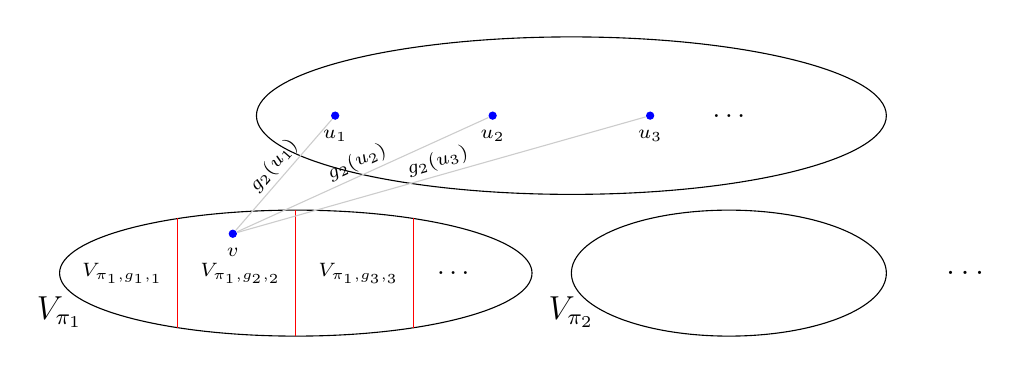
\begin{tikzpicture}
                \draw (0,0) ellipse (4cm and 1cm);
                \node at (-3, 1) {\large $\cH$}; 

                \node[circle,fill=blue,inner sep=0pt,minimum size=3pt,label=below:{\scriptsize $u_1$}] (v1) at (-3, 0) {};
                \node[circle,fill=blue,inner sep=0pt,minimum size=3pt,label=below:{\scriptsize $u_2$}] (v2) at (-1, 0) {};
                \node[circle,fill=blue,inner sep=0pt,minimum size=3pt,label=below:{\scriptsize $u_3$}] (v3) at ( 1, 0) {};
                \node at ( 2, 0) {$\ldots$}; 

                \draw (-3.5, -2) ellipse (3cm and 0.8cm);
                \node at (-6.5,-2.5) {\large $V_{\pi_1}$}; 

                \node at (-5.7,-2) {\scriptsize $V_{\pi_1, \tuple{g_1, \bff_1}}$};
                \node at (-4.2,-2) {\scriptsize $V_{\pi_1, \tuple{g_2, \bff_2}}$};
                \node at (-2.7,-2) {\scriptsize $V_{\pi_1, \tuple{g_3, \bff_3}}$};
                \node at (-1.5,-2) {$\ldots$}; 
                \draw[red] (-5,  -1.3) -- (-5,  -2.7);
                \draw[red] (-3.5,-1.2) -- (-3.5,-2.8);
                \draw[red] (-2,  -1.3) -- (-2,  -2.7);

                \node[circle,fill=blue,inner sep=0pt,minimum size=3pt,label=below:{\scriptsize $v$}] (u) at (-4.3, -1.5) {};

                \draw[gray!40] (v1) --  node[color=black,above=-2,sloped] {\scriptsize $g_2(u_1)$} (u);
                \draw[gray!40] (v2) --  node[color=black,above=-2,sloped] {\scriptsize $g_2(u_2)$} (u);
                \draw[gray!40] (v3) --  node[color=black,above=-2,sloped] {\scriptsize $g_2(u_3)$} (u);

                \draw (2, -2) ellipse (2cm and 0.8cm);
                \node at (0,-2.5) {\large $V_{\pi_2}$}; 

                \node at (5,-2) {\large $\ldots$}; 
            \end{tikzpicture}
        \end{center}
        \caption{An illustration of the model construction extending the partial model $\cH$  for the proof of Theorem~\ref{lem:c2_spec_core}.}
        \label{fig:construct}
    \end{figure}


    \textbf{\uline{Suppose that $\bfv \in \sol{\Psi^\varphi_\cH(\bfx)}$}}.
    For every $\pi \in \onetypes^\varphi$ and
    $\tuple{g, \bff} \in \cB^\varphi_{\pi, \cH}$,
    let $a_\pi$ be the $\pi^{th}$ component of $\bfv$ and
    $b_{\pi, \tuple{g, \bff}}$ be the corresponding assignment to $\bfy$.
    Our goal is to construct a finite model $\cG$ of $\varphi$ by extending the partial model $\cH$.
    The construction is illustrated in Figure~\ref{fig:construct}.
    We extend the partial model $\cH$ by introducing sets of fresh vertices $V_{\pi, \tuple{g, \bff}}$,
    where the cardinality of each set is $b_{\pi, \tuple{g, \bff}}$.
    All vertices in $V_{\pi, \tuple{g, \bff}}$ are assigned the 1-type $\pi$.
    Let $V_{\pi}$ be the union of $V_{\pi, \tuple{g, \bff}}$ for every $\tuple{g, \bff}$.

    We handle edge coloring using a four-step procedure which we now outline.
    Firstly, we
    color edges between the core $\cH$ and the relative complement of the core $\cG \setminus \cH$.
    In steps two and three,
    we iterate over all pairs of 1-types $\pi_1$ and $\pi_2$ realized in the relative complement of the core $\cG \setminus \cH$ and color edges between $V_{\pi_1}$ and $V_{\pi_2}$ as follows:
    \begin{itemize}
        \item In step 2, we color edges with 2-types that are neither forward-silent nor backward-silent.
        \item In step 3, we color edges with 2-types that are not forward-silent,  but which are backward-silent.
    \end{itemize}
    We mention that the following invariant will be maintained during the iteration described above:

    \medskip

    For every $\pi \in \onetypes^\varphi$ and $\tuple{g, \bff} \in \cB^\varphi_{\pi, \cH}$,
    for every vertex $v$ in $V_{\pi, \tuple{g, \bff}}$,
    for every $\pi' \in \onetypes^\varphi$ and $\eta \in \cKvpf_{\pi, \pi'} \cup \cKvpfb_{\pi, \pi'}$,
    the number of colored edges from $v$ to $V_{\pi'}$ with 2-type $\eta$ is either 0 or $\bff(\eta, \pi')$.

    \medskip

    After the iteration, in step 4 we handle the remaining edges with 2-types that are both forward- and backward-silent.
    
    We now provide the details of the procedure.
    \begin{enumerate}
        \item 
            For every $v$ in $\cG \setminus \cH$  and $u$ in $\cH$,
            we add an edge between $v$ and $u$ with 2-type $g(u)$.
        \item
            For every $\pi_1, \pi_2 \in \onetypes^\varphi$,
            we assign audible 2-types in $\cKvpfb_{\pi_1, \pi_2}$ and $\cKvpfb_{\pi_2, \pi_1}$
            between $V_{\pi_1}$ and $V_{\pi_2}$.
            We first assume that parallel edges are allowed,
            Because $b_{\pi, \tuple{g, \bff}}$ is a solution of $\match_{1, \cH}(\bfy)$,
            it is straightforward to assign (parallel) edges between $V_{\pi_1}$ and $V_{\pi_2}$ 
            such that
            \begin{itemize}
            \item
                for every $v \in V_{\pi_1, \tuple{g, \bff}}$, for every $\eta \in \cKvpfb_{\pi_1, \pi_2}$,
                the number of edges from $v$ to $V_{\pi_2}$ with 2-type $\eta$ is exactly $\bff(\eta, \pi_2)$.
            \item
                for every $v \in V_{\pi_2, \tuple{g, \bff}}$, for every $\eta \in \cKvpfb_{\pi_2, \pi_1}$,
                the number of edges from $v$ to $V_{\pi_1}$ with 2-type $\eta$ is exactly $\bff(\eta, \pi_1)$.
            \end{itemize}

            To eliminate parallel edges in the above construction,
            we again apply a swapping procedure, as in \cite{tonyeryk,ultimatelyperiodic}.
            Note that each vertex $v \in V_{\pi_1} \cup V_{\pi_2}$ is adjacent to at most $K^\varphi$ edges.
            Suppose that there are parallel edges $e_1$ and $e_2$
            between $v_1 \in V_{\pi_1}$ and $v_2 \in V_{\pi_2}$ with the 2-type of $e_1$ being $\eta_1$ and
            the $2$-type of $e_2$ being $\eta_2$.
            Let $u_1 \in V_{\pi_1}$ and $u_2 \in V_{\pi_2}$ be vertices such that
            there is an edge $e_3$ between them with 2-type $\eta_2$,
            $u_1$ is not adjacent to $v_2$, and
            $u_2$ is not adjacent to $v_1$.
            Because $b_{\pi, \tuple{g, \bff}}$ is a solution of $\bige_{\cH}(\bfy)$,
            there are at least $(2K^\varphi+1)^2$ edges from $V_{\pi_1}$ to $V_{\pi_2}$ with 2-type $\eta_2$.
            Since each of $v_1$ and $v_2$ has at most $K^\varphi$ adjacent edges,
            it is always possible to find such $u_1$ and $u_2$.
            We then remove the edges $e_2$ and $e_3$,
            and replace them with fresh edges $(v_1, u_2)$ and $(v_2, u_1)$ with 2-type $\eta_2$.
            This swapping procedure preserves the number of edges connected to vertices with specific 2-types
            but reduces the number of parallel edges by 1,
            We can repeat this until all parallel edges are eliminated.

        \item
            For every $\pi_1, \pi_2 \in \onetypes^\varphi$,
            we assign backward-silent but not forward-silent 2-types in $\cKvpf_{\pi_1, \pi_2}$ and $\cKvpf_{\pi_2, \pi_1}$
            between $V_{\pi_1}$ and $V_{\pi_2}$.
            Again, we assume first that parallel edges are allowed,
            Because $b_{\pi, \tuple{g, \bff}}$ is a solution of $\match_{2, \cH}(\bfy)$,
            if $\sum_{\tuple{g, \bff} \in \cB^\varphi_{\pi_1, \cH}} \bff(\eta, \pi_2) \cdot b_{\pi_1, \tuple{g, \bff}} > 0$,
            then $\sum_{\tuple{g, \bff} \in \cB^\varphi_{\pi_2, \cH}} b_{\pi_2, \tuple{g, \bff}} > 0$,
            which implies that $V_{\pi_2}$ is not empty.
            Thus we can assign (parallel) edges from $V_{\pi_1}$ and $V_{\pi_2}$ satisfying that
            \begin{itemize}
            \item
                for every $v \in V_{\pi_1, \tuple{g, \bff}}$, for every $\eta \in \cKvpf_{\pi_1, \pi_2}$,
                the number of edges from $v$ to $V_{\pi_2}$ with 2-type $\eta$ is exactly $\bff(\eta, \pi_2)$.
            \end{itemize}
            A similar argument applies to edges from $V_{\pi_2}$ to $V_{\pi_1}$.
            \begin{itemize}
            \item
                for every $v \in V_{\pi_2, \tuple{g, \bff}}$, for every $\eta \in \cKvpf_{\pi_2, \pi_1}$,
                the number of edges from $v$ to $V_{\pi_1}$ with 2-type $\eta$ is exactly $\bff(\eta, \pi_1)$.
            \end{itemize}

            We apply the swapping procedure to eliminate parallel edges as well.
            Suppose that there are parallel edges $e_1$ and $e_2$
            between $v_1 \in V_{\pi_1}$ and $v_2 \in V_{\pi_2}$ with 2-types $\eta_1 \in \cKvpf_{\pi_1, \pi_2}$ for $e_1$ and $\eta_2$ for $e_2$.
            We consider two cases:
            \begin{itemize}
            \item 
                If there is a vertex $u_2 \in V_{\pi_2}$ such that there is no edges between $v_1$ and $u_2$,
                then we remove $e_1$ and add an edge between $v_1$ and $u_2$ with 2-types $\eta_1$.
            \item 
                Otherwise, suppose that there is no such $u_2$,
                which implies that for every vertex $u \in V_{\pi_2}$,
                there exists an edge $e_3$ between $v_1$ and $u$.
                Because there are at most $2K^\varphi(2K^\varphi+1)^2$ edges
                between $V_{\pi_1}$ and $V_{\pi_2}$,
                we can find $u_1 \in V_{\pi_1}$ and $u_2 \in V_{\pi_2}$
                such that no edges exists between them,
                and there exists an edge $e_3$ between $v_1$ and $u_2$ with type $\eta_3 \in \cKvpb_{\pi_1, \pi_2}$. 
                We then remove the edges $e_1$ and $e_3$
                and fresh edges $(v_1, u_2)$ with 2-type $\eta_1$ and $(v_2, u_2)$ with 2-type $\eta_3$.
            \end{itemize}
            For both cases, the swapping procedure preserves the number of edges connected to vertices with specific 2-types
            but reduces the number of parallel edges by 1,
            We can repeat it until all parallel edges are eliminated.

        \item
            Finally, for every pair of vertices $v_1 \in V_{\pi_1}$ and $v_2 \in V_{\pi_2}$ 
            with no edge connected,
            we add an edge between them with a 2-type  $\eta \in \cKvpnull_{\pi_1, \pi_2}$.
    \end{enumerate}

    We first claim that the 1-type cardinality vector of $\cG$ is exactly $\bfv$.
    For every $\pi \in \onetypes^\varphi$,
    recall that the number of vertices in $\cH$ with 1-type $\pi$ is $s_\pi$.
    The number of vertices in $\cG \setminus \cH$ with 1-type $\pi$ is
    $\abs{V_\pi} = \sum_{\tuple{g, \bff} \in \cB^\varphi_{\pi, \cH}} \abs{V_{\pi, \tuple{g, \bff}}} = \sum_{\tuple{g, \bff} \in \cB^\varphi_{\pi, \cH}} b_{\pi, \tuple{g, \bff}}$.
    Since $a_\pi$ and $b_{\pi, \tuple{g, \bff}}$ is a solution of $\summ_{\cH}(\bfx, \bfy)$,
    we have $a_\pi = s_\pi + \sum_{f \in \cB^\varphi_{\pi, \cH}} b_{\pi, \tuple{g, \bff}}$.
    Recall that $a_\pi$ is the $i^{th}$ component of $\bfv$, where $i$ is the index of $\pi$ in the  ordering of $\onetypes^\varphi$.
    Thus the 1-type cardinality vector of $\cG$ is exactly $\bfv$.

    We next claim that $\cG$ is a model of $\varphi$, by checking the conditions in Proposition~\ref{prop:ctwo_graph}.
    It is routine to check that all vertices and edges in $\cG$ satisfy the 1- and 2-type conditions.
    Thus it is sufficient to check that the counting condition holds for every vertex $v$ in $\cG$.
    \begin{itemize}
        \item
        For every $v$ in $\cH$, note that
        \begin{equation*}
            \sum_{u \in V_{\pi, \tuple{g, \bff}}} \twotypeof^\trif(v, u) 
            \ =\ 
            \sum_{u \in V_{\pi, \tuple{g, \bff}}} g^\trib(v)
            \ =\ 
            g^\trib(v) \cdot \abs{V_{\pi, \tuple{g, \bff}}}
            \ =\ 
            g^\trib(v) \cdot b_{\pi, \tuple{g, \bff}}.
        \end{equation*}
        Because $b_{\pi, \tuple{g, \bff}}$ is a solution of $\comp_{\cH}(\bfy)$, we have
        \begin{equation*}
            \begin{aligned}
                \sum_{u \in V \setminus \set{v}} \twotypeof^\trif(v, u)
                \ =\ &
                \sum_{u \in V_c \setminus \set{v}} \twotypeof^\trif(v, u) +
                \sum_{\pi \in \onetypes^\varphi}\sum_{\tuple{g, \bff} \in \cB^\varphi_{\pi, \cH}}\sum_{u \in V_{\pi, \tuple{g, \bff}}} \twotypeof^\trif(v, u) \\
                \ =\ &
                \sum_{u \in V_c \setminus \set{v}} \twotypeof^\trif(v, u) +
                \sum_{\pi \in \onetypes^\varphi}\sum_{\tuple{g, \bff} \in \cB^\varphi_{\pi, \cH}} g^\trib(v)\cdot b_{\pi, \tuple{g, \bff}} \\
                \ =\ &
                \bfk^\varphi
            \end{aligned}
        \end{equation*}

        \item
        For every $v \in V_{\pi, \tuple{g, \bff}}$,
        note that the extended behavior of $v$ is $\tuple{g, \bff}$.
        Since $\tuple{g, \bff} \in \cB^\varphi_{\pi, \cH}$,
        by the compatibility condition in Definition~\ref{def:compatextended}, it holds that
        \begin{equation*}
            \begin{aligned}
                \sum_{u \in V \setminus \set{v}} \twotypeof^\trif(v, u)
                \ =\ &
                \sum_{u \in V_c} \twotypeof^\trif(v, u) +
                \sum_{u \in V \setminus (V_c \cup \set{v})} \twotypeof^\trif(v, u) \\
                \ =\ &
                \sum_{u \in V_c} g^\trif(u) + 
                \sum_{\pi' \in \onetypes^\varphi}
                \left(
                    \sum_{\eta \in \cKvpf_{\pi, \pi'}} \bff(\eta, \pi') \cdot \eta^\trif +
                    \sum_{\eta \in \cKvpfb_{\pi, \pi'}} \bff(\eta, \pi') \cdot \eta^\trif
                \right) \\
                \ =\ &\bfk^\varphi
            \end{aligned}
        \end{equation*}
    \end{itemize}
\end{proof}

\section{Extensions to modulus constraints}

Recall that in the body of the paper, cardinality constraints, either within $\GPtwo$ or the global cardinality constraints added to $\Ctwo$, did not constrain the modulus of a count. So, for example, in $\GPtwo$ we could not state that the number of neighbors of an element with a given property is even. And similarly, we could not add to $\Ctwo$ a  constraint that the total number of elements in a model satisfying a formula is an even number. We stated in the body that we can add such modulus constraints and obtain the same results.

In this appendix we will first indicate how to extend the satisfiability result for $\GPtwo$ to the case when existential quantifiers are allowed in the Presburger quantifiers, i.e., when the formula $P(x)$ is of the form:
\begin{equation*}
P_i(x)\ :=\ 
\exists x_1 \cdots \exists x_n\ \sum_{t \in \intsinterval{m}} \lambda_{t} \cdot \presby{R_t(x, y) \land x \neq y}
\ + \ \sum_{t\in \intsinterval{n}} \lambda_t'\cdot x_t
\ \circledast_i\ \delta.
\end{equation*}
Note that the existential variables captures a modulus equation, as $a \equiv b \bmod p$ can be rewritten as:
$$
\exists x_1\exists x_2\
a+x_1p = b+x_2p
$$

We claim that Theorem~\ref{thm:gptwoexp} still holds under such a generalization.
The proof is basically the same.
The only difference is that in the definition of characteristic system
$\cC^\varphi_\pi(\bfx)$
defined in Definition~\ref{def:characteristic-system} the variables $\bfx$ include all the existential variables.
Similarly for the system $\cQ^\varphi(\bfx)$
defined in Definition~\ref{def:linear-system-Q}.
Then, we observe that
Lemmas~\ref{lem:equiv1},~\ref{lem:equiv2}, and~\ref{lem:equiv3} still hold for such systems
and the satisfiability problem of $\GPtwo$ stays in $\exptime$.

For the extension of $\Ctwo$ with global cardinality and modulus constraints, the situation is more obvious. We have already shown how to get a (modulus-constraint free) semilinear representation for the type spectrum vectors. We can compose this with modulus constraints in addition to linear arithmetic constraints and solve using standard techniques for Presburger arithmetic. 
Rewriting modulus constraint into a single linear equation does not change the number of constraints in each disjunct in the formula $\Psi^{\varphi}(\bfx)$.
We emphasize again that the argument here is completely generic, and the same comment holds to show that for \emph{any} decidability extension of Presburger arithmetic (e.g. B\"uchi Arithemetic or Semenov Arithmetic \cite{semenovpresexp}), $\Ctwo$ with global cardinality constraints of that form is decidable.


\section*{Expressiveness separation of the considered languages}
We mentioned that the languages we consider in this paper -- $\GPtwo$ and $\Ctwo$ with global cardinality constraints -- are incomparable in expressiveness.

$\GPtwo$  contains sentences not in $\Ctwo$ with constraints, because (as we showed in the paper) the spectrum of GP2 may not be semilinear, while for $\Ctwo$ with constraints the specctrum is always semilinear.

On the other hand, even ordinary $\Ctwo$ contains sentences not in $\GPtwo$: just consider the sentence restricting the cardinality of the model to some fixed number, like $2$. In $\GPtwo$ every sentence that is consistent has models of unbounded finite cardinality, since we can always clone a connected component without disturbing the truth value of any sentence.
